\documentclass[2pt,-letter paper]{article}
\usepackage{graphicx} % Required for inserting images
\usepackage{siunitx}
\usepackage{setspace}
\usepackage{gensymb}
\usepackage{xcolor}
\usepackage{caption}
%\usepackage{subcaption}
\doublespacing
\singlespacing
\usepackage[none]{hyphenat}
\usepackage{amssymb}
\usepackage{relsize}
\usepackage[cmex10]{amsmath}
\usepackage{mathtools}
\usepackage{amsmath}
\usepackage{commath}
\usepackage{amsthm}
\interdisplaylinepenalty=2500
%\savesymbol{iint}
\usepackage{txfonts}
%\restoresymbol{TXF}{iint}
\usepackage{wasysym}
\usepackage{amsthm}
\usepackage{mathrsfs}
\usepackage{txfonts}
\let\vec\mathbf{}
\usepackage{stfloats}
\usepackage{float}
\usepackage{cite}
\usepackage{cases}
\usepackage{subfig}
%\usepackage{xtab}
\usepackage{longtable}
\usepackage{multirow}
%\usepackage{algorithm}
\usepackage{amssymb}
%\usepackage{algpseudocode}
\usepackage{enumitem}
\usepackage{mathtools}
%\usepackage{eenrc}
%\usepackage[framemethod=tikz]{mdframed}
\usepackage{listings}
%\usepackage{listings}
\usepackage[latin1]{inputenc}
%%\usepackage{color}{   
%%\usepackage{lscape}
\usepackage{textcomp}
\usepackage{titling}
\usepackage{hyperref}
%\usepackage{fulbigskip}   
\usepackage{tikz}
\usepackage{graphicx}
\lstset{
  frame=single,
  breaklines=true
}
\let\vec\mathbf{}
\usepackage{enumitem}
\usepackage{graphicx}
\usepackage{siunitx}
\let\vec\mathbf{}
\usepackage{enumitem}
\usepackage{graphicx}
\usepackage{enumitem}
\usepackage{tfrupee}
\usepackage{amsmath}
\usepackage{amssymb}
\usepackage{mwe} % for blindtext and example-image-a in example
\usepackage{wrapfig}
\graphicspath{{images/}}
\providecommand{\mydet}[1]{\ensuremath{\begin{vmatrix}#1\end{vmatrix}}}
\providecommand{\myvec}[1]{\ensuremath{\begin{bmatrix}#1\end{bmatrix}}}
\providecommand{\cbrak}[1]{\ensuremath{\left\{#1\right\}}}
\providecommand{\brak}[1]{\ensuremath{\left(#1\right)}}
\title{MATHEMATICS}
\author{}
\begin{document}
\maketitle


\date{\today}
\begin{enumerate}


\section{NUMBER SYSTEM}

\item Find after how many places of decimal the decimal form of the number $\frac {27}{2^3.5^4.3^2}$ will terminate.

\item Express $429$ as a product of its prime factors.

\item If HCF of $65$ and $117$ is expressible in the form $65n - 117$, then find the value of $n$.

\item On a morning walk, three persons step out together and their steps measure $30 cm$, $36 cm$ and $40 cm$ respectively. What is the minimum distance each should walk so that each can cover the same distance in complete steps ?

\item Prove that $\sqrt{3}$ is an irrational number.

\item Find the largest number which on dividing $1251$, $9377$ and $15628$ leaves remainders $1$, $2$ and $3$ respectively.\\

\section{ALGEBRA}

\item Write the discriminant of the quadratic equation $\brak {x + 5}^2 = 2 \brak {5x {-3}}$.

\item Find the sum of first $10$ multiples of $6$

\item Solve the following pair of linear equations :
\begin{align*}
 3x - 5y = 4\\
2y + 7 = 9x   
\end{align*}    

\item Using completing the square method, show that the equation
$x^2 - 8x + 18 = 0$ has no solution.

\item Check whether $g\brak{x}$ is a factor of $p\brak{x}$ by dividing polynomial $p\brak{x}$ by polynomial $g\brak{x}$,where $p\brak{x} = x^5 - 4x^3 + x^2 + 3x + 1$ , $g\brak{x} = x^3 - 3x + 1$

\item If $m$ times the $m^{th}$ term of an Arithmetic Progression is equal to $n$ times
its $n^{th}$ term and $m \neq n$, show that the $\brak{m + n}^{th}$ term of the A.P is zero

\item The sum of the first three numbers in an Arithmetic Progression is $18$. If the product of the first and the third term is $5$ times the common
difference, find the three numbers.


\item  Solve the following pair of linear equations :
\begin{align*}
3x + 4y = 10\\
2x - 2y = 2
\end{align*}

\item If $\frac{2}{3}$ and $-3$ are the zeroes of the polynomial $ax^2 + 7x + b$, then find the values of $a$ and $b$.\\

\section{COORDINATE GEOMETRY}

\item Find the value $\brak{s}$ of $x$, if the distance between the points $A\brak{0, 0}$ and $B \brak{x,-4}$  is $5$ units.

\item Points $A\brak{3, 1}, B\brak{5, 1},C\brak{a, b}$ and $D\brak{4, 3}$ are vertices of a parallelogram $ABCD$. Find the values of $a$ and $b$.

\item Points $P$ and $Q$ trisect the line segment joining the points $A\brak{-2, 0}$ and $B\brak{0, 8}$ such that $P$ is near to $A$. Find the coordinates of points $P$ and $Q$.

\item Find the area of the triangle formed by joining the mid-points of the sides of the triangle ABC, whose vertices are $A\brak{0, - 1}$, $B\brak{2, 1}$ and $C\brak{0, 3}$.

\item Draw the graph of the equations $x - y + 1 = 0$ and $3x + 2y - 12 = 0$. Using this graph, find the values of $x$ and $y$ which satisfy both the equations.

\item Find the value of $k$ so that the area of triangle $ABC$ with $A\brak{k + 1, 1}$, $B\brak{4, -3}$ and $C\brak{7, -k}$ is $6$ square units.\\

\section{TRIGONOMETRY}

\item In \figref{fig:Fig_1}, $PS = 3 cm$, $QS = 4 cm$, $\angle$ $PRQ$ = $\theta$, $\angle$ $PSQ$ = $90\degree$, $PQ$ $\perp$ $RQ$ and $RQ = 9 cm$. Evaluate $\tan$ $\theta$.
\begin{figure}[H]
    \centering
    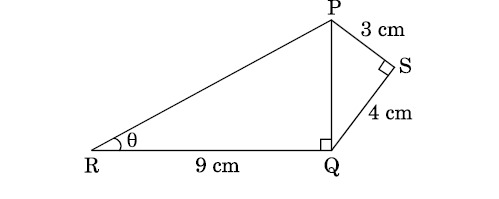
\includegraphics[width=\columnwidth]{Screenshot2023-12-27094821.png}
     \caption{Triangle PSQR}
    \label{fig:Fig_1}
\end{figure}



\item If $\tan$ $\alpha$ = ${\frac {5}{12}}$, find the value of $\sec$ $\alpha$.

\item $A$, $B$ and $C$ are interior angles of a triangle $ABC$. Show that
\begin{enumerate}
\item  $\sin$ $ \brak{{\frac {B+C}{2}}} = \cos {\frac {A}{2}}$
\item  If $\angle A = 90 \degree$ , then find the value of $\tan \brak{{\frac{B+C}{2}}}$ 
\end{enumerate} 

\item If $\tan \brak{A + B} = 1$ and $\tan \brak{A - B} = \frac{1}{\sqrt{3}}$ , $0\degree$ $<$ $A + B$ $<$ $90\degree$, $A > B$, then find the values of $A$ and $B$.

\item If $1 + \sin^2 \theta  = 3 \sin \theta \cos \theta$, then prove that $\tan$ $\theta = 1 $ or $\tan$ $\theta = \frac{1}{2}$

\item The shadow of a tower standing on a level ground is found to be $40 m$ longer when the Sun's altitude is $30\degree$ than when it was $60\degree$. Find the height of the tower. $(Given \sqrt{3} = 1.732)$

\item Prove that in a right triangle, the square of the hypotenuse is equal to the sum of the squares of the other two sides.

\item Prove that :
\begin{align*}
\frac{\tan^3 \theta}{1+\tan^2 \theta} + \frac{\cot^3 \theta}{1 + \cot^2 \theta} =  \sec \theta  \csc  \theta - 2 \sin \theta \cos \theta  
\end{align*}\\

\section{GEOMETRY}

\item Two concentric circles of radii $a$ and $b$ $\brak{a > b}$ are given. Find the length of the chord of the larger circle which touches the smaller circle.

\item The perpendicular from $A$ on side $BC$ of a $\triangle ABC$ meets $BC$ at $D$ such that
$DB = 3CD$. Prove that $2AB^2 = 2AC^2 + BC^2$.

\item $AD$ and $PM$ are medians of triangles $ABC$ and $PQR$ respectively where
$\triangle ABC \sim \triangle PQR$. Prove that ${\frac {AB}{PQ}} = {\frac {AD}{PM}}$.

\item In \figref{fig:Fig_2}, PQ is a chord of length $8 cm$ of a circle of radius $5 cm$. The tangents at $P$ and $Q$ intersect at a point $T$. Find the length $TP$.
\begin{figure}[H]
    \centering
    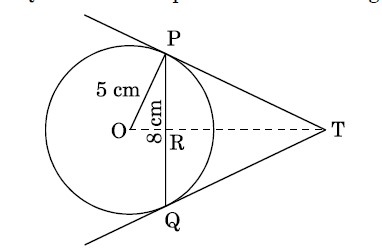
\includegraphics[width=\columnwidth]{Screenshot2023-12-27160239.png}
    \caption{CIRCLE}
    \label{fig:Fig_2}
\end{figure}


\item Prove that opposite sides of a quadrilateral circumscribing a circle subtend supplementary angles at the centre of the circle.

\item A pole has to be erected at a point on the boundary of a circular park of diameter $13 m$ in such a way that the difference of its distances from two
diametrically opposite fixed gates $A$ and $B$ on the boundary is $7 m$. Is it possible to do so ? If yes, at what distances from the two gates should the pole be erected ?

\item A chord of a circle of radius $14 cm$ subtends an angle of $60\degree$ at the centre. Find the area of the corresponding minor segment of the circle.
$({Use \hspace{4pt}\pi=\frac{22}{7} and \sqrt{3} = 1.732})$

\item Construct a triangle, the lengths of whose sides are $5 cm$, $6 cm$ and $7 cm$. Now construct another triangle whose sides are $\frac{5}{7}$ times the corresponding sides of the first triangle.

\item If a line is drawn parallel to one side of a triangle to intersect the other two sides in distinct points, prove that the other two sides are divided in the same ratio.

\item Construct a triangle $ABC$ with side $BC = 6 cm$, $AB = 5 cm$ and $\angle ABC = 60\degree$. Then construct another triangle whose sides are $\frac{3}{4}$ of the corresponding sides of the triangle $ABC$

\section{MENSURATION}

\item Water in a canal, $6 m$ wide and $1.5 m$ deep, is flowing with a speed of $10 km/h $. How much area will it irrigate in $30$ minutes if $8 cm$ of standing water is needed?

\item A car has two wipers which do not overlap. Each wiper has a blade of length $21 cm$ sweeping through an angle $120\degree$. Find the total area cleaned at each sweep of the blades. $(Take  \pi=\frac{22}{7})$

\item In \figref{fig:Fig_3}, a decorative block is shown which is made of two solids, a cube and a hemisphere. The base of the block is a cube with edge $6 cm $ and the hemisphere fixed on the top has a diameter of $4.2 cm $. Find
 \begin{enumerate}
 \item  the total surface area of the block.
 \item the volume of the block formed.$(Take  \pi=\frac{22}{7})$
 \end{enumerate}
\begin{figure}[H]
    \centering
    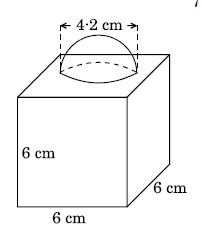
\includegraphics[width=\columnwidth]{image.png}
    \caption{CUBE AND HEMISPHERE}
    \label{fig:Fig_3}
\end{figure}

\item A bucket open at the top is in the form of a frustum of a cone with a capacity of $12308.8 cm^3 $. The radii of the top and bottom circular ends are $20 cm $ and $12 cm $ respectively. Find the height of the bucket and the area of metal sheet used in making the bucket.$(Use \pi=3.17)$

\item A motorboat whose speed in still water is $9 km/h $, goes $15km$ downstream and comes back to the same spot, in a total time of $3 hours$ $45 minutes$. Find the speed of the stream.

\section{PROBABILITY}

\item A die is thrown once. Find the probability of getting
\begin{enumerate}
\item a composite number,
\item a prime number.
\end{enumerate}

\item Cards numbered $7$ to $40$ were put in a box. Poonam selects a card at
random. What is the probability that Poonam selects a card which is a
multiple of $7$ ?


\end{enumerate}

\end{document}
